\documentclass[12pt,a4paper,openright,twoside]{report}
\usepackage[italian,english]{babel}
\usepackage{fancyhdr}
\usepackage{indentfirst}
\usepackage{newlfont}
\usepackage{pdfpages}
\usepackage{abstract}
\usepackage{tabularx}
\usepackage{colortbl}
\usepackage{multirow}
\usepackage{graphicx}
\usepackage{listings}
\usepackage{subcaption}
\usepackage[hidelinks]{hyperref}
\definecolor{background}{HTML}{EEEEEE}
\lstdefinelanguage{json}{
    basicstyle=\footnotesize\ttfamily,
    numbers=left,
    numberstyle=\ttfamily,
    stepnumber=1,
    numbersep=8pt,
    showstringspaces=false,
    breaklines=true,
    backgroundcolor=\color{background}
}
\graphicspath{ {./images/} }
\oddsidemargin=30pt \evensidemargin=20pt
\pagestyle{fancy}\addtolength{\headwidth}{20pt}\setlength{\headheight}{15pt}
\renewcommand{\chaptermark}[1]{\markboth{\thechapter.\ #1}{}}
\renewcommand{\sectionmark}[1]{\markright{\thesection \ #1}{}}
\rhead[\fancyplain{}{\bfseries\leftmark}]{\fancyplain{}{\bfseries\thepage}}
\cfoot{}
\linespread{1.3}
\begin{document}
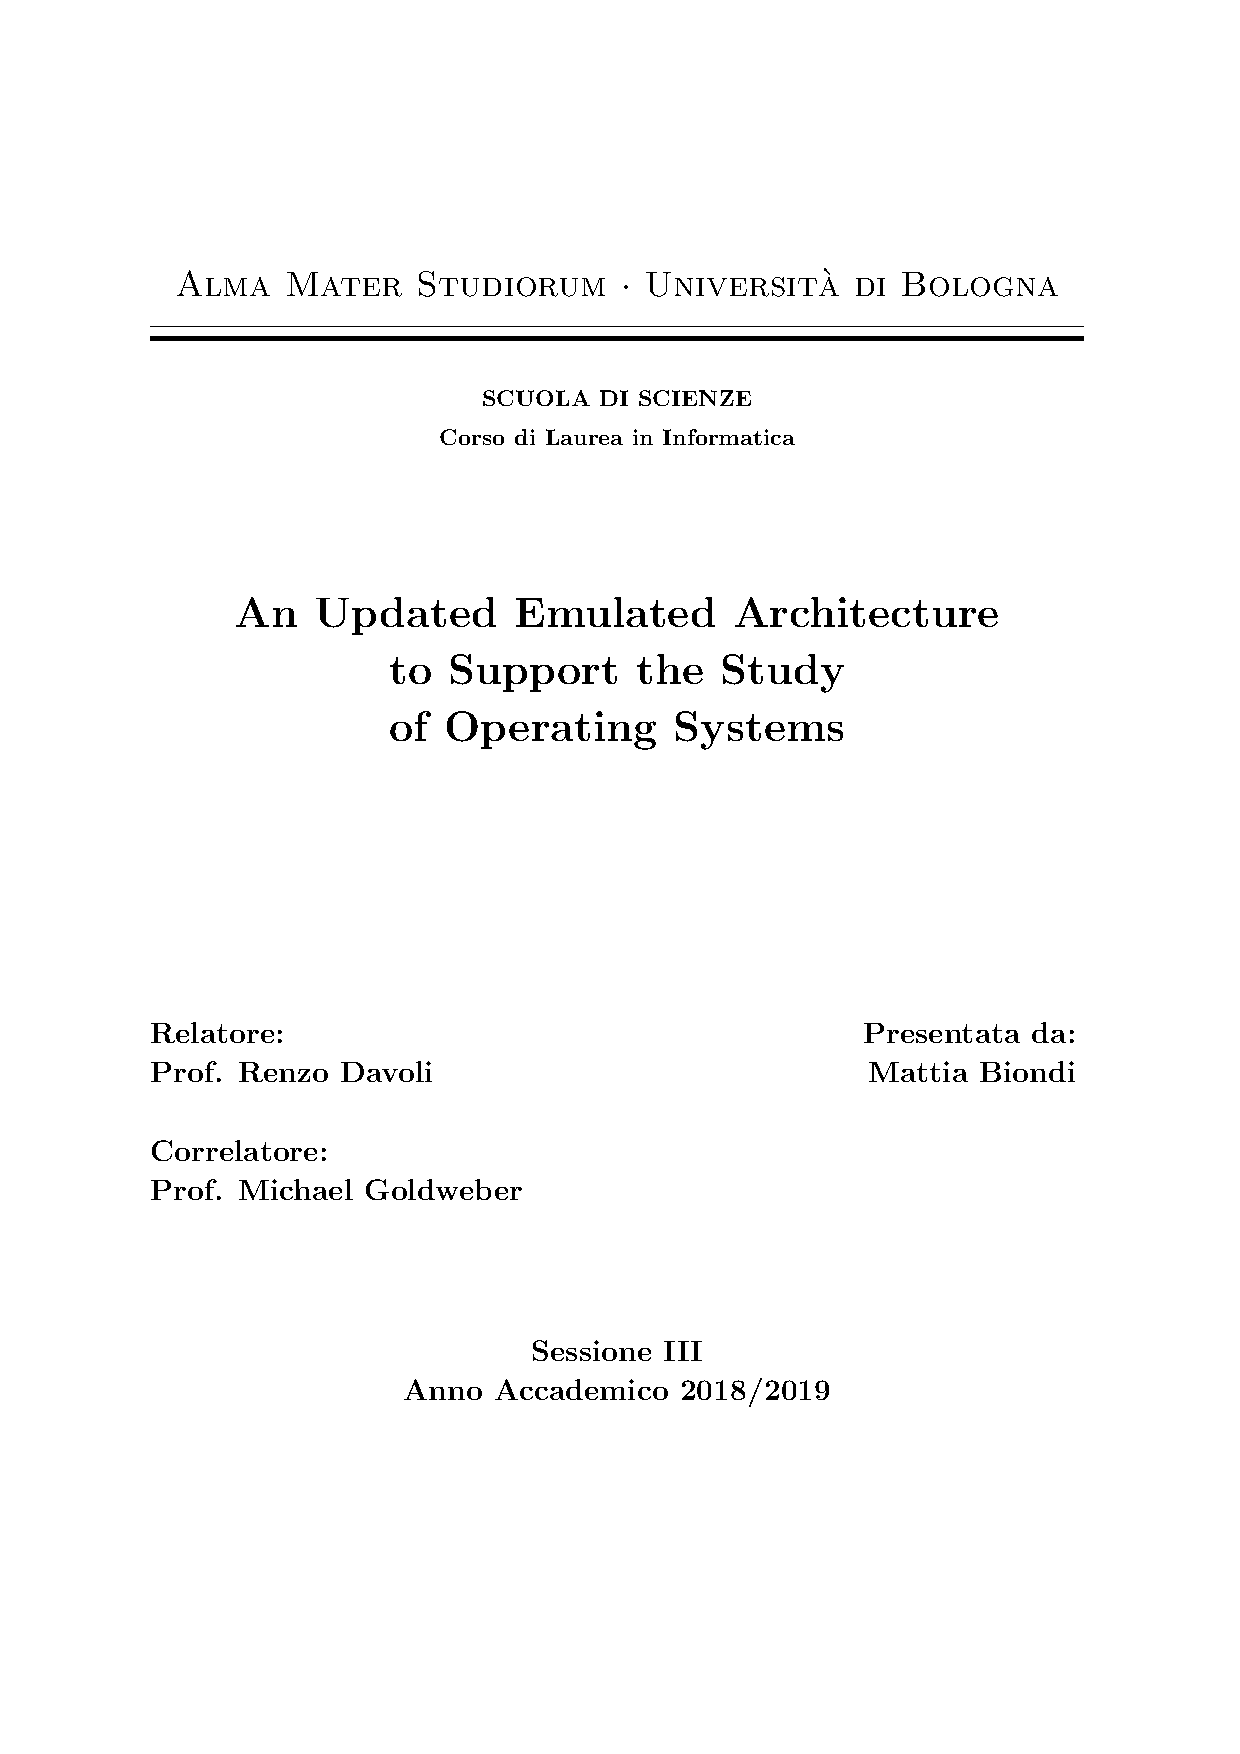
\includepdf[pages=-]{titlepage.pdf}
\clearpage{\pagestyle{empty}\cleardoublepage}
\begin{titlepage}
	\thispagestyle{empty}
	\topmargin=6.5cm
	\raggedleft
	\large
	\em
	dedica

	\newpage
	\clearpage{\pagestyle{empty}\cleardoublepage}
\end{titlepage}
\begin{abstract}
	\pagenumbering{roman}
	One of the most effective ways to learn something new is by actively practising it, and there is---maybe---no better way to study an Operating Systems course than by building your OS.

	However, it is important to emphasize how the realization of an operating system capable of running on a real hardware machine could be an overly complex and unsuitable task for an undergraduate student.
	Nonetheless, it is possible to use a simplified computer system simulator to achieve the goal of teaching Computer Science foundations in the university environment, thus allowing students to experience a quite realistic representation of an operating system.

	$\mu$MPS has been created for this purpose, a pedagogically appropriate machine emulator, based around the MIPS R2/3000 microprocessor, which features an accessible architecture that includes a rich set of easily programmable devices.
	$\mu$MPS has an almost two decades old historical development and the outcome of this following thesis is the third version of the software, dubbed $\mu$MPS3.
	This second major revision aims to simplify, even more, the emulator’s complexity in order to lighten the load of work required by the students during the OS design and implementation.
	Two of these simplifications are the removal of the virtual memory bit, which allowed address translation to be turned on and off, and the replacement of the tape device, used as storage devices, with a new flash drive device---certainly something more familiar to the new generation of students.

	Thanks to the employment of this software and the feed-backs received over the last decade, it has been possible to realize not just this following thesis, but also to develop some major improvements, which concern everything from the project building tools to the front-end, making $\mu$MPS a modern and reliable educational software.
\end{abstract}
\clearpage{\pagestyle{empty}\cleardoublepage}
\selectlanguage{italian}
\begin{abstract}
	\setcounter{page}{3}
	Uno dei metodi più efficaci per imparare qualcosa di nuovo è facendo pratica, e probabilmente, non esiste modo migliore di studiare un corso di Sistemi Operativi, se non scrivendo il proprio SO.
	È tuttavia necessario prendere atto di quanto la realizzazione di un sistema operativo, in grado di girare su una vera macchina hardware, sia un compito eccessivamente complesso e quasi inadeguato per uno studente universitario.
	Ciò non toglie che sia però possibile far uso di simulatori di sistemi semplificati rispetto alla realtà, al fine di riuscire nell'insegnamento dei fondamenti dell'Informatica in contesti universitari, permettendo così agli studenti di sperimentare con una rappresentazione di un sistema operativo abbastanza realistica.

	$\mu$MPS è stato sviluppato proprio a questo scopo, un emulatore di sistemi pedagogicamente appropriato, basato sul microprocessore MIPS R2/3000, e dotato di un'architettura accessibile e di un ricco lista di dispositivi facilmente programmabili.
	$\mu$MPS conta quasi vent'anni di sviluppo, ora aggiornato tramite la seguente tesi alla sua terza versione, chiamata $\mu$MPS3.
	Quest'ultimo aggiornamento mira a semplificare, ancor di più, la complessità dell'emulatore, al fine di alleggerire il carico di lavoro richiesto agli studenti durante lo sviluppo e l'implementazione del sistema operativo.
	Due di queste semplificazioni sono la rimozione del bit di memoria virtuale, che permetteva l'attivazione e la disattivazione della traduzione di indirizzi, e la sostituzione dei nastri, utilizzati come dispositivi di archiviazione, con delle nuove unità di memoria flash---certamente più familiari alla nuova generazione di studenti.

	Grazie all'utilizzo di questo software e dei feedback ricevuti, nel corso degli ultimi dieci anni, è stato possibile non solo realizare la seguente tesi, ma anche apportare alcune importanti migliorie che riguardano tutti i campi, dagli strumenti di compilazione del progetto alla parte front-end, rendendo così $\mu$MPS un software pedagogico moderno e affidabile.
\end{abstract}
\clearpage{\pagestyle{empty}\cleardoublepage}
\selectlanguage{english}
\tableofcontents
\addtocontents{toc}{\protect\thispagestyle{empty}}
\listoffigures
\clearpage{\pagestyle{empty}\cleardoublepage}
\listoftables
\clearpage{\pagestyle{empty}\cleardoublepage}
\lstlistoflistings
\clearpage{\pagestyle{empty}\cleardoublepage}

\chapter*{Notational Conventions}
\begin{itemize}
	\item Words being defined are \textit{italicized};
	\item A \texttt{typewriter-like typeface} is used for memory addresses, machine registers, instructions, file names, identifiers, and code fragments;
	\item Memory addresses and operation codes are given in hexadecimal and displayed in big-endian format;
	\item Bits of storage are numbered right-to-left, starting with 0;
	\item All diagrams illustrating memory are going from low addresses to high addresses, using a left to right, bottom to top orientation.
\end{itemize}

\clearpage{\pagestyle{empty}\cleardoublepage}
\pagenumbering{arabic}
\chapter{Introduction}
\lhead[\fancyplain{}{\bfseries\thepage}]{\fancyplain{}{\bfseries\rightmark}}

\section{Background}
The study and the consequent implementation of how an operating system works is, by now, a long-established and consolidated practice in every Computer Science's curriculum.
It is, actually, one of the crucial components of a computer and it is responsible of ensuring it's basic operations, by coordinating and managing the system's resources like processor, memory, devices and processes, thus allowing hardware and software to interface each other.

This is probably the first real example of ``big project'' which students must experience, thanks to complex intercommunication system that has to exist between the different machine's components, and the study of it allows to comprehend the most common software engineering practices.

The approach on practical contexts is essential to fully understand how a machine works behind the theoretical notions studied in the early stages of the course of study, and it is usually followed by the debate of which is the best teaching choice concerning processor architectures.

Obviously, there is not only one way of how a central processor unit can be implemented, and while older realizations---although applicable for educational purposes---are now obsolete and incompatible with current platforms, modern ones are designed to achieve high speed and quality, which makes them overly complex and unsuitable for the pedagogic experience.

Over the years, the MIPS architecture has become one of the landmarks in this teaching choice due to its clean and elegant instruction set, despite being excessively convoluted to student’s perception, because of the high level of details obscuring the basic underlying features of it.
A potential solution to this problem is the adoption of a simplified computer system simulator, like $\mu$MPS, to bring together an adequate level of understanding and a realistic representation of a real operating system.

\section{History of $\mu$MPS}
$\mu$MPS is based on the machine emulator MPS \cite{mps}, designed and realized by Professor Renzo Davoli and one of his graduate students Mauro Morsiani, in the late 1990s at the University of Bologna.

The initial purpose was to bring back to life the layout and implementation experience of an operating system through an educational emulator, which could be run on real hardware.
This practice was already possible in the past years, when the processor's architecture studied were the same available on real machines, but it has gone lost through the years because of the high-speed development of new more complex technologies used on physical implementations.

MPS was able to emulate the MIPS R3000 processor along with five other different device categories: disks, tapes, network adapters, printers and terminals.

The concerned CPU was genuinely emulated together with its complex virtual memory management system, which was the main subject of the feed-backs received during class testing of MPS as a pedagogical tool at the University of Bologna and Xavier University, in an undergraduate operating systems courses, taught respectively by Renzo Davoli and Michael Goldweber.

It was tested through \textit{Kaya}'s \cite{kaya} implementation, one of the variety of graduate-level projects that the emulator can support.

The urge of simplification led to the creation of $\mu$MPS, virtually identical to MPS but with the addition of a virtual memory management subsystem which had to resemble as much as possible to the conceptual one found in popular introductory OS texts.
The only other difference was the new novice-friendly graphical user interface, significantly improved again in 2011 by Tomislav Jonjic during the development of the first major revision of the emulator, $\mu$MPS2 \cite{umps2}, which also implemented the support to up to sixteen MIPS R3000-style processors.

\section{$\mu$MPS3}
More than ten years have passed since the first release of $\mu$MPS and as many have passed from the moment it has been developed into a consolidated educational tool in the two already acknowledged teaching courses.

As already mentioned, the students' observations during this period were essential to in-depth testing the $\mu$MPS emulator as a pedagogical tool, showing as a result that further changes were needed.
Some examples of these modifications would be the memory's structure and management system of both physical and virtual ones, a nuance probably still too complex and confusing, which could feel like a regression, since the attempt to simplify it has led to the removal of the VM bit.
This was originally introduced in the first version of $\mu$MPS, as a distinctive feature from its predecessor MPS.
On the other hand, other changes are related to the passage of the years, such as the replacement of memory tapes with flash drive devices, also know as ``USB sticks'' or ``SD cards''.

Tapes are probably still studied in their operation nowadays, but they cannot be found in today's practical contexts, and therefore it could be difficult to understand for the new generation of students, who can't find a match in current technological implementations.

Another consequence of $\mu$MPS's modernization has been the shift from the historical and well established Autotools to a more modern building tool, CMake, that speeds up the compilation process in addition to simplify the project's structure.
It also fits best with the current emulator's graphical user interface, originally built upon Qt4, which also undergoes to the migration to the new version, Qt5.

These and more changes are collected together in a major release of the project, $\mu$MPS3, consequently bringing even more reliability in terms of pedagogical tool.

Due to implementation aspects---unlike his predecessor $\mu$MPS2---this new version is not backward compatible with older ones.

\texttt{TODO: Debian Packaging}

\section{Document's Structure}

\chapter{Memory Management}
\lhead[\fancyplain{}{\bfseries\thepage}]{\fancyplain{}{\bfseries\rightmark}}
Like for the two prior versions, the memory subsystem of $\mu$MPS3 is divided into two views: physical and virtual.
Both parts have undergone significant modifications in this major revision, and they will be described in detail in this chapter, alongside their old versions and respective changes.

The main reasons for the modifications made are the further simplification of the work required by the user for the kernel implementation and the better clarification of the emulator's memory internal view, which, in the past, have caused some difficulties to the students.

\section{Physical Memory}
The physical address space is divided into two big areas [\autoref{fig:physical_memory}]: a \textit{kernel reserved space}, from address \texttt{0x0000.0000} to \texttt{0x2000.0000}, and the \textit{installed RAM}, from address \texttt{0x2000.0000} (\texttt{RAMBASE}) to \texttt{RAMTOP}.

This last value is calculated upon the one retrieved from the configuration file, settable from the machine's configuration dialog in the front-end emulator, which goes from a minimum of 8 to a maximum of 512 memory frames.
Being the size of each frame 4 kilobyte, $\mu$MPS3 can have from 32KB up to 2MB of installed RAM.
Hence, the value of \texttt{RAMTOP} range from \texttt{0x2000.8000} to \texttt{0x2020.0000}.

\begin{figure}[ht]
	\centering
	\begin{tabular}{cl}
		                                                             & \multirow{2}{*}{\texttt{0xFFFF.FFFF}} \\ \cline{1-1}
		\multicolumn{1}{|c|}{\multirow{2}{*}{\cellcolor{gray}}}      &                                       \\ [-1ex]
		\multicolumn{1}{|c|}{\cellcolor{gray}}                       & \multirow{2}{*}{\texttt{RAMTOP}}      \\ \cline{1-1}
		\multicolumn{1}{|c|}{\multirow{4}{*}{installed RAM}}         &                                       \\
		\multicolumn{1}{|c|}{}                                       &                                       \\
		\multicolumn{1}{|c|}{}                                       &                                       \\
		\multicolumn{1}{|c|}{}                                       & \multirow{2}{*}{\texttt{0x2000.0000}} \\ \cline{1-1}
		\multicolumn{1}{|c|}{\multirow{2}{*}{kernel reserved space}} &                                       \\
		\multicolumn{1}{|c|}{}                                       & \multirow{2}{*}{\texttt{0x0000.0000}} \\ \cline{1-1}
		\multicolumn{1}{l}{}                                         &
	\end{tabular}
	\caption{Physical Memory}
	\label{fig:physical_memory}
\end{figure}

\subsection{Kernel Reserved Space}
\label{chap:kernel_reserved_space}
The first memory's big area [\autoref{fig:kernel_reserved_space}] is reserved for:
\begin{itemize}
	\item the Execution ROM code, which lays in a read-only segment from address \texttt{0x0000.0000} to \texttt{ROMTOP}. This latter value is calculated upon the size of the Execution ROM;
	\item the BIOS Data Page, from address \texttt{0x0FFF.F000} (\texttt{BIOSDATABASE}) to \texttt{0x1000.0000}. This is a new area that has been implemented in a $\mu$MPS2's unused memory space.
	      See \autoref{chap:bios_data_page} for more information regarding this read/writable area segment;
	\item the Bus Register Area, from address \texttt{0x1000.0000} to \texttt{0x1000.002C}: a 11 words area that will be described later in \autoref{chap:tlb_floor_address};
	\item the Installed Devices Bit Map, from address \texttt{0x1000.002C} to \\ \texttt{0x1000.0040}: a read-only five words area that indicates which devices are actually installed and where [\texttt{TODO} of \cite{pops}];
	\item the Interrupting Devices Bit Map, from address \texttt{0x1000.0040} to \\ \texttt{0x1000.0054}: a read-only five words area that indicates which devices have an interrupt pending [\texttt{TODO} of \cite{pops}];
	\item the Devices' Registers Area, from address \texttt{0x1000.0054} to \texttt{0x1000.02D4} (\texttt{DEVTOP}): a 160 words area (number of interrupt lines (8) $\times$ devices per interrupt line (5) $\times$  words per register (4)). See \texttt{TODO} of \cite{pops} for more information, or \autoref{tab:device_register_layout} for an example of one device's register;
	\item the Bootstrap ROM code, which lays in a read-only segment from address \texttt{0x1FC0.0000} to \texttt{BOOTTOP}. This latter value is calculated upon the size of the Bootstrap ROM.
\end{itemize}
\begin{figure}[ht]
	\centering
	\renewcommand{\arraystretch}{0.95}
	\begin{tabular}{cl}
		\multicolumn{1}{l}{}                                                & \multirow{2}{*}{\texttt{0x2000.0000}} \\ \cline{1-1}
		\multicolumn{1}{|l|}{\cellcolor{gray}}                              &                                       \\ [-3ex]
		\multicolumn{1}{|l|}{\cellcolor{gray}}                              & \multirow{2}{*}{\texttt{BOOTTOP}}     \\ \cline{1-1}
		\multicolumn{1}{|c|}{\multirow{2}{*}{Bootstrap ROM}}                &                                       \\ [-1ex]
		\multicolumn{1}{|c|}{}                                              & \multirow{2}{*}{\texttt{0x1FC0.0000}} \\ \cline{1-1}
		\multicolumn{1}{|l|}{\multirow{2}{*}{\cellcolor{gray}}}             &                                       \\ [-3ex]
		\multicolumn{1}{|l|}{\cellcolor{gray}}                              & \multirow{2}{*}{\texttt{DEVTOP}}      \\ \cline{1-1}
		\multicolumn{1}{|c|}{\multirow{2}{*}{Devices' Register Area}}       &                                       \\ [-1ex]
		\multicolumn{1}{|c|}{}                                              & \multirow{2}{*}{\texttt{0x1000.0054}} \\ \cline{1-1}
		\multicolumn{1}{|c|}{\multirow{2}{*}{Interrupting Devices Bit Map}} &                                       \\ [-1ex]
		\multicolumn{1}{|c|}{}                                              & \multirow{2}{*}{\texttt{0x1000.0040}} \\ \cline{1-1}
		\multicolumn{1}{|c|}{\multirow{2}{*}{Installed Devices Bit Map}}    &                                       \\ [-1ex]
		\multicolumn{1}{|c|}{}                                              & \multirow{2}{*}{\texttt{0x1000.002C}} \\ \cline{1-1}
		\multicolumn{1}{|c|}{\multirow{2}{*}{Bus Register Area}}            &                                       \\ [-1ex]
		\multicolumn{1}{|c|}{}                                              & \multirow{2}{*}{\texttt{0x1000.0000}} \\ \cline{1-1}
		\multicolumn{1}{|c|}{\multirow{2}{*}{BIOS Data Page}}               &                                       \\ [-1ex]
		\multicolumn{1}{|c|}{}                                              & \multirow{2}{*}{\texttt{0x0FFF.F000}} \\ \cline{1-1}
		\multicolumn{1}{|l|}{\multirow{2}{*}{\cellcolor{gray}}}             &                                       \\ [-3ex]
		\multicolumn{1}{|l|}{\cellcolor{gray}}                              & \multirow{2}{*}{\texttt{ROMTOP}}      \\ \cline{1-1}
		\multicolumn{1}{|c|}{\multirow{2}{*}{Execution ROM}}                &                                       \\ [-1ex]
		\multicolumn{1}{|c|}{}                                              & \multirow{2}{*}{\texttt{0x0000.0000}} \\ \cline{1-1}
		\multicolumn{1}{l}{}                                                &
	\end{tabular}
	\caption{Kernel Reserved Space's Structure}
	\label{fig:kernel_reserved_space}
\end{figure}
Any attempt to access an undefined memory area (\texttt{ROMTOP...0x0FFF.F000}, \texttt{DEVTOP...0x1FC0.0000}, \texttt{BOOTTOP...0x2000.0000}) will generate a \textit{Bus Error exception} [\autoref{chap:exception_handling}].

Note: the memory area between address \texttt{0x1000.02D4} (\texttt{DEVTOP}) and \texttt{0x1FC0.0000} is not completely undefined [section 7.3 of \cite{old_pops}].

\subsection{RAM Space}
The maximum \texttt{RAMTOP} value that could be actually set is \texttt{0x2020.0000}.
However, since $\mu$MPS3 uses 32-bit addresses, it could support up to [$2^{32}$ - \texttt{RAMBASE}] $\simeq$ 3.5GB of RAM.
The 2MB graphical user interface limitation is imposed because, while it seems a ridiculously small amount of memory in today's ordinary systems, it is, actually, a lot more than has ever been required in all these years of $\mu$MPS use.

This area will hold:
\begin{itemize}
	\item the operating system's code (\textit{text}), global variables/structures (\textit{data}), and stack(s);
	\item The user processes' \textit{text}, \textit{data} and stacks.
\end{itemize}
As for the previous big area, any attempt to access the undefined memory area that lays from \texttt{RAMTOP} up to \texttt{0xFFFF.FFFF} will generate a Bus Error exception.

\section{Virtual Memory}
The virtual memory subsystem is implemented through a segmented-paged scheme.
Hence, a new abstraction layer is laid on the whole physical memory structure, subdividing it into four big segments [\autoref{fig:new_segments}]:
\begin{itemize}
	\item \textit{kseg0}, from address \texttt{0x0000.0000} to \texttt{0x2000.0000}: a 0.5GB segment reserved for the Kernel Reserved Space [\autoref{chap:kernel_reserved_space}];
	\item \textit{kseg1}, from address \texttt{0x2000.0000} to \texttt{0x4000.0000}: a 0.5GB segment reserved for OS \textit{text}, \textit{data} and stacks;
	\item \textit{kseg2}, from address \texttt{0x4000.0000} to \texttt{0x8000.0000}: a 1GB segment reserved for OS \textit{text}, \textit{data} and stacks;
	\item \textit{kuseg}, from address \texttt{0x8000.0000} to \texttt{0xFFFF.FFFF}: a 2GB segment reserved for user processes' \textit{text}, \textit{data} and stacks;
\end{itemize}
This subdivision differs from $\mu$MPS2's one, as it was divided in three different segments [\autoref{fig:old_segments}]:
\begin{itemize}
	\item \textit{ksegOS}, from address \texttt{0x0000.0000} to \texttt{0x8000.0000}: a 2GB segment reserved for OS \textit{text}, \textit{data} and stacks, along with all the structures that sit in the kernel reserved space up to address \texttt{0x2000.0000};
	\item \textit{kUseg2}, from address \texttt{0x8000.0000} to \texttt{0xC000.0000}: a 1GB virtual address space reserved for user processes' \textit{text}, \textit{data} and stacks;
	\item \textit{kUseg3}, from address \texttt{0xC000.0000} to \texttt{0xFFFF.FFFF}: another 1GB virtual address space reserved for the use of user-mode processes.
\end{itemize}

\begin{figure}[h]
	\centering
	\begin{subfigure}[b]{0.4\textwidth}
		\renewcommand{\arraystretch}{0.66}
		\begin{tabular}{cl}
			\multicolumn{1}{m{3cm}}{}                     & \multirow{2}{*}{\texttt{0xFFFF.FFFF}} \\ \cline{1-1}
			\multicolumn{1}{|c|}{\multirow{2}{*}{kUseg3}} &                                       \\
			\multicolumn{1}{|c|}{}                        & \multirow{2}{*}{\texttt{0xC000.0000}} \\ \cline{1-1}
			\multicolumn{1}{|c|}{\multirow{2}{*}{kUseg2}} &                                       \\
			\multicolumn{1}{|c|}{}                        & \multirow{2}{*}{\texttt{0x8000.0000}} \\ \cline{1-1}
			\multicolumn{1}{|c|}{\multirow{8}{*}{ksegOS}} &                                       \\
			\multicolumn{1}{|c|}{}                        & \multirow{2}{*}{}                     \\
			\multicolumn{1}{|c|}{}                        &                                       \\
			\multicolumn{1}{|c|}{}                        & \multirow{2}{*}{}                     \\
			\multicolumn{1}{|c|}{}                        &                                       \\
			\multicolumn{1}{|c|}{}                        & \multirow{2}{*}{}                     \\
			\multicolumn{1}{|c|}{}                        &                                       \\
			\multicolumn{1}{|c|}{}                        & \multirow{2}{*}{\texttt{0x0000.0000}} \\ \cline{1-1}
			\multicolumn{1}{l}{}                          &
		\end{tabular}
		\caption{Old Segments}
		\label{fig:old_segments}
	\end{subfigure}
	\qquad
	\qquad
	\begin{subfigure}[b]{0.4\textwidth}
		\renewcommand{\arraystretch}{0.66}
		\begin{tabular}{cl}
			\multicolumn{1}{m{3cm}}{}                    & \multirow{2}{*}{\texttt{0xFFFF.FFFF}} \\ \cline{1-1}
			\multicolumn{1}{|c|}{\multirow{4}{*}{kuseg}} &                                       \\
			\multicolumn{1}{|c|}{}                       & \multirow{2}{*}{}                     \\
			\multicolumn{1}{|c|}{}                       &                                       \\
			\multicolumn{1}{|c|}{}                       & \multirow{2}{*}{\texttt{0x8000.0000}} \\ \cline{1-1}
			\multicolumn{1}{|c|}{\multirow{4}{*}{kseg2}} &                                       \\
			\multicolumn{1}{|c|}{}                       & \multirow{2}{*}{}                     \\
			\multicolumn{1}{|c|}{}                       &                                       \\
			\multicolumn{1}{|c|}{}                       & \multirow{2}{*}{\texttt{0x4000.0000}} \\ \cline{1-1}
			\multicolumn{1}{|c|}{\multirow{2}{*}{kseg1}} &                                       \\
			\multicolumn{1}{|c|}{}                       & \multirow{2}{*}{\texttt{0x2000.0000}} \\ \cline{1-1}
			\multicolumn{1}{|c|}{\multirow{2}{*}{kseg0}} &                                       \\
			\multicolumn{1}{|c|}{}                       & \multirow{2}{*}{\texttt{0x0000.0000}} \\ \cline{1-1}
			\multicolumn{1}{l}{}                         &
		\end{tabular}
		\caption{New Segments}
		\label{fig:new_segments}
	\end{subfigure}
	\caption{Virtual Address Space}
	\label{fig:virtual_address_space}
\end{figure}

The first 2GB of physical memory, corresponding to all the addresses below \texttt{0x8000.0000}, were and are reserved only to kernel-mode access, therefore, any attempt to access them while the processor is in user-mode will cause the raising of an \textit{Address Error} [\autoref{chap:exception_handling}].

The other half of memory is, now, dedicated to user processes, and each one ``sees'' his own virtual version.
One process' kuseg is separated from another process' one by a unique number called \textit{ASID} (Address Space Identifier) [\texttt{TODO} of \cite{pops}].

In previous versions, wether this subdivision was active or not, it was controlled by the \textit{VM bit}.
With the VM bit off, no particular actions were required when accessing the memory space.
Instead, when the VM bit was on, all the address above \texttt{0x2000.0000} were considered virtual, and therefore subject to \textit{virtual address translation}---the process to associate a non-accessible address to a physical one.
By doing this, instead of the actual physical memory available, the processes perceive an abstract view of the address space.

The virtual address translation process went through a significant change in this major revision: the formal segment table and page table formats [subsections 4.3.1 and 4.3.2 of \cite{old_pops}], introduced in the first implementation of $\mu$MPS, have been removed, resulting in a simpler procedure for the users [\texttt{TODO} of \cite{pops}].

During the implementation of a new emulator's feature, the VM bit has been completely removed too.

\subsection{VM Bit Removal}
\label{chap:vm_bit_removal}
The VM bit was originally introduced in the first version of $\mu$MPS, with the intent of simplifying the complex virtual memory management system of the MIPS R3000 microprocessor.
The activation and deactivation of it was accomplished through the system control coprocessor \textit{CP0}.

It provides a 32-bit \textit{Status} register that controls various aspects of the emulator, described in details at \texttt{TODO} of \cite{pops}.
Along with the current register's options set, it also provided the possibility, by using bitwise operations, to control the VM bit's status: it was implemented as a 3-slot deep bit stack (current, previous, previous of previous) which was pushed or popped depending on whether an exception was raised or an interrupted execution stream was restarted [section 3.2 and subsection 6.2.1 of \cite{old_pops}].

The VM bit removal is one of $\mu$MPS3's main features: the push/pop system has been removed, and the three bits that were reserved for it are now completely ignored.
Hence, from now on, the virtual memory is conceptually \textbf{always on}.
This means that all the addresses above a certain value are considered virtual and therefore, subject to virtual address translation.
This specific value, while in previous version was fixed at \texttt{0x2000.0000}, is now contained in a variable called \textit{TLB Floor Address}

\subsection{TLB Floor Address}
\label{chap:tlb_floor_address}
The TLB Floor Address is a new parameter implemented in $\mu$MPS3, responsible for indicating which addresses from a certain value on are considered virtual.

This parameter can be chosen directly from the configuration dialog in the emulator's front-end, as Figure \ref{fig:tlb_floor_address} shows:
\begin{figure}[h]
	\centering
	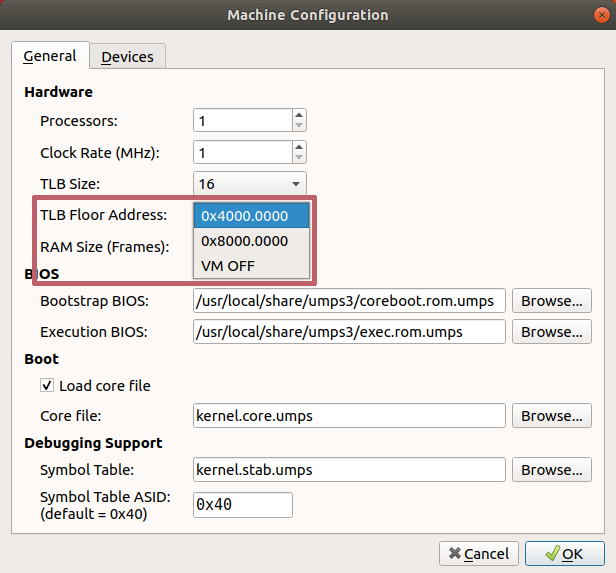
\includegraphics[scale=0.73]{tlb_floor_address}
	\caption{TLB Floor Address}
	\label{fig:tlb_floor_address}
\end{figure}

The last option, \texttt{VM OFF}, is internally declared as \texttt{0xFFFF.FFFF}: since it is not possible to access to an address above this value, the entire physical memory is necessarily below it, and therefore, an address translation could never happen.

The TLB Floor Address value is stored in the Bus Register Area, thereby adding one word to the ten words area of the previous version [\autoref{tab:bus_register_area}]:
\begin{table}[h]
	\centering
	\renewcommand{\arraystretch}{0.98}
	\begin{tabular}{|c|c|}
		\hline
		Physical Address     & Field Name                          \\ \hline\hline
		\texttt{0x1000.0000} & RAM Base Physical Address           \\ \hline
		\texttt{0x1000.0004} & Installed RAM Size                  \\ \hline
		\texttt{0x1000.0008} & Exec. ROM Base Physical Address     \\ \hline
		\texttt{0x1000.000C} & Installed Exec. ROM Size            \\ \hline
		\texttt{0x1000.0010} & Bootstrap ROM Base Physical Address \\ \hline
		\texttt{0x1000.0014} & Installed Bootstrap ROM Size        \\ \hline
		\texttt{0x1000.0018} & Time of Day Clock - High            \\ \hline
		\texttt{0x1000.001C} & Time of Day Clock - Low             \\ \hline
		\texttt{0x1000.0020} & Interval Timer                      \\ \hline
		\texttt{0x1000.0024} & Time Scale                          \\ \hline
		\texttt{0x1000.0028} & \textbf{TLB Floor Address}          \\ \hline
	\end{tabular}
	\caption{Bus Register Area}
	\label{tab:bus_register_area}
\end{table}

This area contains various fields used in $\mu$MPS3's lifetime cycle to properly work.
Some of them are read-only and calculated at boot/reset time, while others are read/writable.
See \texttt{TODO} of \cite{pops} for more information regarding this area.

The TLB Floor Address's field cannot be changed while the emulator is running, but only from the front-end dialog.

After saving the machine's configuration from the front-end dialog, the TLB Floor Address's value will be placed inside the JSON-based configuration's file, described in detail in subsection 4.2.1 of Jonjic's Thesis \cite{tjonjic}.

An example of the final portion of a simple machine's configuration is represented in Listing \ref{lst:tlb_floor_adress}:
\begin{lstlisting}[language=json,firstnumber=19,caption={TLB Floor Address},captionpos=b,label={lst:tlb_floor_adress}]
    ...
    },
    "tlb-floor-address": "0x40000000",
    "tlb-size": 16
  }
  \end{lstlisting}
On line 21 is shown the value saved as \textit{string}: this decision was taken to preserve the human-readable notational convention, used across all $\mu$MPS3's environment, consisting of addresses written in hexadecimal base, preceded by the ``\texttt{0x}'' prefix.

One of the consequences of the implementation of this value at the end of the Bus Register Area has been the shifting up of one word of the two successive areas, Installed Devices Bit Map and Interrupting Devices Bit Map.

\chapter{Exception Handling}
\label{chap:exception_handling}
\lhead[\fancyplain{}{\bfseries\thepage}]{\fancyplain{}{\bfseries\rightmark}}
Exceptions are particular events that interrupt a machine's normal flow of execution.
Different categories of them exist, each one raised in correspondence of a certain occurrence.
Depending on their type, the exceptions require to be handled in a distinct special way rather than with the ordinary system's workflow.

$\mu$MPS3 supports four different types of exceptions:
\begin{itemize}
	\item \textit{Program Traps}: these exceptions are usually raised when the user-defined workflow commits an error, like: \textit{Address Error}, \textit{Bus Error}, \textit{Reserved Instruction}, \textit{Coprocessor Unusable} or \textit{Arithmetic Overflow};
	\item \textit{System Calls and Breakpoints}: these two occur whenever a process request an OS service through the \texttt{SYSCALL} or the \texttt{BREAK} instruction;
	\item \textit{Interrupts}: I/O devices that complete their previously started operation must notify it to the processor, and they do it by raising this type of exception. There are a total of 8 interrupt lines: 3 of them are dedicated to internally generated interrupts, while the other 5 to external devices. Each of these last five ones support up to 8 devices attached to them;
	\item \textit{TLB-related exceptions}: exceptions linked to the \textit{Translation Lookaside Buffer}: \textit{TLB-Modification}, \textit{TLB-Invalid} and \textit{TLB-Refill}.
\end{itemize}

Going more in details on Program Traps, from \texttt{TODO} of \cite{pops}:
\begin{quote}
	\begin{itemize}
		\item Address Error is raised when:
		      \begin{itemize}
			      \item a load/store/instruction fetch of a word is not aligned on a word boundary;
			      \item a load/store of a half-word is not aligned on a halfword boundary;
			      \item a user-mode access is made to an address below \texttt{0x8000.0000};
		      \end{itemize}
		\item Bus Error is raised whenever an access is attempted on a non-existent physical memory location or when an attempt is made to write onto ROM storage;
		\item Reserved Instruction is raised whenever an instruction is ill-formed, not recognizable, or it is privileged and executed while in user-mode;
		\item Coprocessor Unusable is raised whenever an instruction requiring the use of (or access to) an uninstalled or currently unavailable coprocessor is executed;
		\item Arithmetic Overflow is raised whenever an \texttt{ADD} or \texttt{SUB} instruction execution results in a 2's complement overflow;
	\end{itemize}
\end{quote}

The TLB (Translation Lookaside Buffer) is a Virtual Memory management system's component whose functioning has not changed since last $\mu$MPS' version.
However, its exception handling did, and, therefore, a little background is needed to explain the modifications made. From \texttt{TODO} of \cite{pops}:
\begin{quote}
	The TLB is an \textit{associative cache}, that can hold from 4 to 64 TLB entries.
	Each TLB entry describes the mapping between one ASID–virtual page number pairing and a physical frame number/location in RAM.
	By utilizing a cache of recently used TLB entries, $\mu$MPS3's virtual address translation mechanism can avoid making multiple memory accesses for each translation by linearly searching the TLB for a matching entry.
\end{quote}

Hence, regarding its exceptions, from \texttt{TODO} of \cite{pops}:
\begin{quote}
	\begin{itemize}
		\item TLB-Modification is raised when on a write request a ``matching'' entry is found, the entry is marked valid, but not dirty/writable;
		\item TLB-Invalid is raised whenever a ``matching'' entry is found but the entry is marked invalid;
		\item TLB-Refill is raised when no ``matching'' entry is found.
	\end{itemize}
\end{quote}

\section{Processor Actions on Exception}
When an exception is raised, the processor's state (what it was ``doing'') must be saved in order to restart from that point after the exception has been handled.
Before doing this, the processor has to take a number of atomic actions (non-interruptible, without any visible intermediary state).
Some fundamental steps are, then:
\begin{itemize}
	\item disabling all interrupts, to make sure nothing could disturb the entire handling process;
	\item activating the kernel-mode, since the access to the memory area intended for saving (and retrieving) the processor's state is denied to user-mode processes.
\end{itemize}
In addition to these, another step to disable the virtual memory was taken in $\mu$MPS' previous versions, since the processor's state reserved area was above the address \texttt{0x2000.0000}.
With the virtual memory bit enabled, those addresses were considered virtual, leading to possible raises of TLB-management exceptions, which would have meant entering in an \textit{infinite loop}.
However, as explained in \autoref{chap:vm_bit_removal}, this has been completely removed in $\mu$MPS3.

Other essential processor actions are taken, some of them based on the type of the exception.
They remain unchanged from $\mu$MPS2, and explained in detail in \texttt{TODO} of \cite{pops}.
This chapter will focus on the differences between the two versions and the modifications made.

\section{Previous Implementation}
The exception handling of $\mu$MPS' previous versions was managed by distinguishing them by their type: Program Traps, System Calls and Breakpoints, Interrupts and TLB-related exceptions.

Since this subdivision existed, four different areas were needed to save the processor's state (called \textit{old areas}), and other four to retrieve the state to be loaded (called \textit{new areas}), which contained the address of the exception's handler.
These four pair of areas, each one linked to its specific exception's type, were stored in a 35 (state's size) $\times$ 8 words area [\autoref{fig:old_new_state_areas}] at the beginning of the so-called \textit{ROM Reserved Frame} [\autoref{fig:rom_reserved_frame}].

\subsection{ROM Reserved Frame}
\begin{figure}[h]
	\centering
	\begin{subfigure}[b]{0.4\textwidth}
		\renewcommand{\arraystretch}{0.83}
		\begin{tabular}{cl}
			\multicolumn{1}{l}{}                                                  & \multirow{2}{*}{\texttt{0x2000.0460}} \\ \cline{1-1}
			\multicolumn{1}{|c|}{\multirow{2}{*}{\begin{tabular}[c]{@{}c@{}}Syscalls and Breakpoints\\ (new area)\end{tabular}}} &                                       \\
			\multicolumn{1}{|c|}{}                                                & \multirow{2}{*}{\texttt{0x2000.03D4}} \\ \cline{1-1}
			\multicolumn{1}{|c|}{\multirow{2}{*}{\begin{tabular}[c]{@{}c@{}}Syscalls and Breakpoints\\ (old area)\end{tabular}}} &                                       \\
			\multicolumn{1}{|c|}{}                                                & \multirow{2}{*}{\texttt{0x2000.0348}} \\ \cline{1-1}
			\multicolumn{1}{|c|}{\multirow{2}{*}{\begin{tabular}[c]{@{}c@{}}Program Traps\\ (new area)\end{tabular}}} &                                       \\
			\multicolumn{1}{|c|}{}                                                & \multirow{2}{*}{\texttt{0x2000.02BC}} \\ \cline{1-1}
			\multicolumn{1}{|c|}{\multirow{2}{*}{\begin{tabular}[c]{@{}c@{}}Program Traps\\ (old area)\end{tabular}}} &                                       \\
			\multicolumn{1}{|c|}{}                                                & \multirow{2}{*}{\texttt{0x2000.0230}} \\ \cline{1-1}
			\multicolumn{1}{|c|}{\multirow{2}{*}{\begin{tabular}[c]{@{}c@{}}TLB-related\\ exceptions (new area)\end{tabular}}} &                                       \\
			\multicolumn{1}{|c|}{}                                                & \multirow{2}{*}{\texttt{0x2000.01A4}} \\ \cline{1-1}
			\multicolumn{1}{|c|}{\multirow{2}{*}{\begin{tabular}[c]{@{}c@{}}TLB-related\\ exceptions (old area)\end{tabular}}} &                                       \\
			\multicolumn{1}{|c|}{}                                                & \multirow{2}{*}{\texttt{0x2000.0118}} \\ \cline{1-1}
			\multicolumn{1}{|c|}{\multirow{2}{*}{\begin{tabular}[c]{@{}c@{}}Interrupt\\ (new area)\end{tabular}}} &                                       \\
			\multicolumn{1}{|c|}{}                                                & \multirow{2}{*}{\texttt{0x2000.008C}} \\ \cline{1-1}
			\multicolumn{1}{|c|}{\multirow{2}{*}{\begin{tabular}[c]{@{}c@{}}Interrupt\\ (old area)\end{tabular}}} &                                       \\
			\multicolumn{1}{|c|}{}                                                & \multirow{2}{*}{\texttt{0x2000.0000}} \\ \cline{1-1}
			\multicolumn{1}{l}{}                                                  &
		\end{tabular}
		\caption{Old and New State Areas}
		\label{fig:old_new_state_areas}
	\end{subfigure}
	\qquad
	\qquad
	\qquad
	\begin{subfigure}[b]{0.4\textwidth}
		\renewcommand{\arraystretch}{0.83}
		\begin{tabular}{cl}
			\multicolumn{1}{l}{}                                                  & \multirow{2}{*}{\texttt{0x2000.0FFF}} \\ \cline{1-1}
			\multicolumn{1}{|c|}{\multirow{2}{*}{\begin{tabular}[c]{@{}c@{}}Stack space for\\ the ROM Routines\end{tabular}}} &                                       \\
			\multicolumn{1}{|c|}{}                                                & \multirow{2}{*}{\texttt{0x2000.0FF0}} \\ \cline{1-1}
			\multicolumn{1}{|c|}{\multirow{4}{*}{\cellcolor{gray}}}               &                                       \\ [3ex]
			\multicolumn{1}{|c|}{\cellcolor{gray}}                                &                                       \\
			\multicolumn{1}{|c|}{\cellcolor{gray}}                                &                                       \\
			\multicolumn{1}{|c|}{\cellcolor{gray}}                                & \multirow{2}{*}{\texttt{0x2000.0800}} \\ \cline{1-1}
			\multicolumn{1}{|c|}{\multirow{4}{*}{64 Segment Tables}}              &                                       \\ [-1ex]
			\multicolumn{1}{|c|}{}                                                & \multirow{2}{*}{}                     \\
			\multicolumn{1}{|c|}{}                                                &                                       \\
			\multicolumn{1}{|c|}{}                                                & \multirow{2}{*}{\texttt{0x2000.0500}} \\ \cline{1-1}
			\multicolumn{1}{|c|}{\multirow{2}{*}{\cellcolor{gray}}}               &                                       \\ [-2ex]
			\multicolumn{1}{|c|}{\cellcolor{gray}}                                & \multirow{2}{*}{\texttt{0x2000.0460}} \\ \cline{1-1}
			\multicolumn{1}{|c|}{\multirow{4}{*}{Old/new areas}}                  &                                       \\
			\multicolumn{1}{|c|}{}                                                & \multirow{2}{*}{}                     \\
			\multicolumn{1}{|c|}{}                                                &                                       \\
			\multicolumn{1}{|c|}{}                                                & \multirow{2}{*}{\texttt{0x2000.0000}} \\ \cline{1-1}
			                                                                      &
		\end{tabular}
		\caption{Overview}
		\label{fig:rom_reserved_frame_overview}
	\end{subfigure}
	\caption{ROM Reserved Frame}
	\label{fig:rom_reserved_frame}
\end{figure}

The ROM Reserved Frame was a 4KB (the size of a frame) area at the beginning of the installed RAM.
It was used, apart from storing the old/new processor's state, also to contain other structures, as \autoref{fig:rom_reserved_frame_overview} shows:
\begin{itemize}
	\item a \textit{Segment Table}, from address \texttt{0x2000.0500} to \texttt{0x2000.0800}: a 64 (number of maximum concurrent processes) $\times$ 3 (number of $\mu$MPS2's segments) words area that contained page table pointers [subsection 4.3.1 of \cite{old_pops}];
	\item a \textit{Stack Space}, from address \texttt{0x2000.0FF0} to \texttt{0x2000.0FFF}, dedicated to the execution of the \textit{ROM exception handlers}.
\end{itemize}

\subsection{ROM Exception Handlers}
The ROM Exception Handlers are routines whose job is to prepare the environment on which the kernel's exception handlers will work.
This means that, after an exception has been raised, before the user-defined functions take place, a series of different actions are made by the ROM (also called \textit{BIOS}), depending on the exception's type.

Apart from some error checking, their essential task is to store off the processor's state in the exact moment the execution's flow has been interrupted in a ``safe place'' in memory (the old areas).
Furthermore, a new state is loaded onto the processor from a previously set area (the new areas), the one containing the kernel's handler, thus ending the ROM's handlers job.

This ``passing'' set of instructions was internally distinguished into two main events' categories: TLB-Refill exceptions, and all the other ones.
The entire new $\mu$MPS3's exception handling system is based on this distinction.

\section{Current Implementation}
\label{chap:new_exception_handling}
Since all the internal exception handling was dealt upon the ``TLB-Refill/all the others'' exceptions separation, the current $\mu$MPS' implementation brings it even to the front, to the user-perceivable part.
Hence, the old processor's state areas have been reduced from four to two, one for each category.

In addition, the kernel's handlers to which pass the control to are no more treated as new states to load onto the processor, but just as functions to which let the \textit{Program Counter} jump to.
This means that the four new processor's state areas are no longer needed too, and has been reduced to only two one-word areas.

Two more one-word areas are needed for the two handlers' stack pointers, so the stack space that was previously reserved at the end of the first frame of RAM has been separated for this purpose.

Finally, the ROM Reserved Frame, previously sat in the first frame of RAM, has been moved to the last frame of memory below the address \texttt{0x1000.0000} (where the Bus Register Area starts), renamed into \textit{BIOS Data Page} [\autoref{fig:bios_data_page}].

\subsection{BIOS Data Page}
\label{chap:bios_data_page}

\begin{figure}[h]
	\centering
	\begin{subfigure}[b]{0.4\textwidth}
		\renewcommand{\arraystretch}{0.77}
		\begin{tabular}{cl}
			\multicolumn{1}{l}{}                                                  & \multirow{2}{*}{\texttt{0x1000.0000}} \\ \cline{1-1}
			\multicolumn{1}{|l|}{\multirow{4}{*}{\cellcolor{gray}}}               &                                       \\ [-2ex]
			\multicolumn{1}{|l|}{\cellcolor{gray}}                                &                                       \\
			\multicolumn{1}{|l|}{\cellcolor{gray}}                                &                                       \\
			\multicolumn{1}{|l|}{\cellcolor{gray}}                                & \multirow{2}{*}{\texttt{0x0FFF.FA00}} \\ \cline{1-1}
			\multicolumn{1}{|c|}{\multirow{3}{*}{\begin{tabular}[c]{@{}c@{}}16$\times$ Handlers'\\ PCs and SPs\end{tabular}}} &                                       \\
			\multicolumn{1}{|c|}{}                                                &                                       \\
			\multicolumn{1}{|c|}{}                                                & \multirow{2}{*}{\texttt{0x0FFF.F900}} \\ \cline{1-1}
			\multicolumn{1}{|c|}{\multirow{2}{*}{\cellcolor{gray}}}               &                                       \\ [-2ex]
			\multicolumn{1}{|c|}{\cellcolor{gray}}                                & \multirow{2}{*}{\texttt{0x0FFF.F8C0}} \\ \cline{1-1}
			\multicolumn{1}{|c|}{\multirow{4}{*}{\begin{tabular}[c]{@{}c@{}}16$\times$ Processor's\\ State Area\end{tabular}}} &                                       \\
			\multicolumn{1}{|c|}{}                                                &                                       \\
			\multicolumn{1}{|c|}{}                                                &                                       \\
			\multicolumn{1}{|c|}{}                                                & \multirow{2}{*}{\texttt{0x0FFF.F000}} \\ \cline{1-1}
			\multicolumn{1}{l}{}                                                  &
		\end{tabular}
		\caption{Overview}
		\label{fig:bios_data_page_overview}
	\end{subfigure}
	\qquad
	\begin{subfigure}[b]{0.4\textwidth}
		\renewcommand{\arraystretch}{1.08}
		\begin{tabular}{cl}
			                                                                      & \multirow{2}{*}{\texttt{0x0FFF.F910}} \\ \cline{1-1}
			\multicolumn{1}{|c|}{\multirow{2}{*}{\begin{tabular}[c]{@{}c@{}}General Exception\\ Stack Pointer\end{tabular}}} &                                       \\
			\multicolumn{1}{|c|}{}                                                & \multirow{2}{*}{\texttt{0x0FFF.F90C}} \\ \cline{1-1}
			\multicolumn{1}{|c|}{\multirow{2}{*}{\begin{tabular}[c]{@{}c@{}}General Exception\\ Handler Address\end{tabular}}} &                                       \\
			\multicolumn{1}{|c|}{}                                                & \multirow{2}{*}{\texttt{0x0FFF.F908}} \\ \cline{1-1}
			\multicolumn{1}{|c|}{\multirow{2}{*}{\begin{tabular}[c]{@{}c@{}}TLB-Refill\\ Stack Pointer\end{tabular}}} &                                       \\
			\multicolumn{1}{|c|}{}                                                & \multirow{2}{*}{\texttt{0x0FFF.F904}} \\ \cline{1-1}
			\multicolumn{1}{|c|}{\multirow{2}{*}{\begin{tabular}[c]{@{}c@{}}TLB-Refill\\ Handler Address\end{tabular}}} &                                       \\
			\multicolumn{1}{|c|}{}                                                & \multirow{2}{*}{\texttt{0x0FFF.F900}} \\ \cline{1-1}
			\multicolumn{1}{l}{}                                                  &
		\end{tabular}
		\caption{Processor 0's Handlers Area}
		\label{fig:four_word_area}
	\end{subfigure}
	\caption{BIOS Data Page}
	\label{fig:bios_data_page}
\end{figure}

The BIOS Data Page is the new $\mu$MPS3's 4KB area reserved for the exception handling.
As \autoref{fig:bios_data_page_overview} shows, it contains:
\begin{itemize}
	\item a \textit{Processors' States Area}, from address \texttt{0x0FFF.F000} to \texttt{0x0FFF.F8C0}: a 35 (state's size) $\times$ 16 (maximum number of active CPUs) words area dedicated to store the state loaded onto one processor at the moment an exception occurred.
	      Since $\mu$MPS2 implemented the multiprocessor support, one area for each active CPU is needed.
	      Processor 0's area is at address \texttt{0x0FFF.F000}, processor 1's one at \texttt{0x0FFF.F08C} (+35 words) and so on;
	\item a \textit{Handlers' Area}, from address \texttt{0x0FFF.F900} to \texttt{0x0FFF.FA00}: a 4 $\times$ 16 words area containing, for each active CPU:
	      \begin{itemize}
		      \item the address of its TLB-Refill handler, to which the workflow will jump after saving the processor's state;
		      \item the TLB-Refill handler's stack pointer;
		      \item the address of its general exceptions handler;
		      \item the general exceptions handler's stack pointer;
	      \end{itemize}
	      \autoref{fig:four_word_area} shows this four-word area for the first processor.
	      As for the previous reserved space, these areas are ordered one after the other, from low to high processors' numbers.
	      Processor 1's one will be at address \texttt{0x0FFF.F910}, processor 2's one at \texttt{0x0FFF.F920} (+4 words) and so on.
\end{itemize}

Note: the 192 words Segment Table area has been completely removed, since it is no longer used in the new address translation process.
\newline

The ROM exception handlers have been updated as well, simplifying the code which was sometimes redundant and in order to comply with the exception handling's changes.

How $\mu$MPS3 knows where to find the right area to save each processors' state and to retrieve the handlers is described along with the updated multiprocessor support in \autoref{chap:multiprocessor_support}.

\chapter{Multiprocessor Support}
\label{chap:multiprocessor_support}
\lhead[\fancyplain{}{\bfseries\thepage}]{\fancyplain{}{\bfseries\rightmark}}
The first major revision, $\mu$MPS2, has implemented the multiprocessor support: the emulator is currently capable of supporting up to 16 simultaneously active CPUs.
Their functioning has not been changed in this new emulator's version, described in detail at chapter 7 of \cite{old_pops}.
However, it is important to understand how their initialization has been modified in order to comply with the new exception handling [\autoref{chap:new_exception_handling}].

\section{Processors Initialization}
As subsection 7.2.2 of \cite{old_pops} explains, each processor has a private set of five \textit{Processor Interface Registers} [\autoref{tab:processor_interface_registers}], and each one sees only its own private instance.
While the first three fields have not changed in their working, the other two have.

\begin{table}[h]
	\centering
	\renewcommand{\arraystretch}{0.85}
	\begin{tabular}{|c|c|c|}
		\hline
		Address              & Register        & Type       \\ \hline\hline
		\texttt{0x1000.0400} & Inbox           & Read/Write \\ \hline
		\texttt{0x1000.0404} & Outbox          & Write Only \\ \hline
		\texttt{0x1000.0408} & TPR             & Read/Write \\ \hline
		\texttt{0x1000.040c} & BIOS Reserved 1 & Read/Write \\ \hline
		\texttt{0x1000.0410} & BIOS Reserved 2 & Read/Write \\ \hline
	\end{tabular}
	\caption{Processor Interface Registers}
	\label{tab:processor_interface_registers}
\end{table}

\subsection{Processor 0}
The first thing that is loaded right after the machine has been turned on (or restarted), is the \textit{Bootstrap ROM} [\texttt{TODO} of \cite{pops}].
It is responsible for setting up the correct handling areas [\autoref{chap:bios_data_page}] for the default processor, the first one.

\textit{BIOS Reserved 1} and \textit{BIOS Reserved 2} are used for this purpose.
For the first processor, the first one was previously set (in the Boostrap code) to the beginning of the Old/New State Area [\autoref{fig:old_new_state_areas}], at address \texttt{0x2000.0000}, while the latter to the stack space at the end of the first frame of RAM, at address \texttt{0x2000.0FFF}.

At boot/reset time, BIOS Reserved 1 is now set up to point to the bottom of the BIOS Data Page [\autoref{fig:bios_data_page}], where its exceptions state's reserved space starts.
On the other hand, BIOS Reserved 2 has now to point to the four-word area reserved for kernel's handlers and their stack pointers, at address \texttt{0x0FFF.F900}. After that, the Bootstrap ROM loads the OS code.

\subsection{Processors 1-15}
How all the other processors were previously initialized is described in subsection 7.1.2 of \cite{old_pops}.

In brief, the \textit{libumps} library provides a ROM service designed to simplify processors' initialization.
Libumps is a C library supplied with the installation of $\mu$MPS to provide access to CP0 instructions, the CP0 registers, and the extended ROM-based services/instructions avoiding to program in MIPS assembler.

This particular function is called \texttt{initCPU} [subsection 7.5.2 of \cite{old_pops}] and the original syntax was:
\begin{verbatim}
  void INITCPU (uint32_t cpuid,
                state_t *start_state,
                state_t *state_areas);
\end{verbatim}

The ROM service's job was to initiate the processor specified by \texttt{cpuid}, loading onto it the processor's state from the supplied \texttt{start\_state} parameter.
The address of BIOS Reserved 2 was calculated by multiplying the processor's number $\times$ the size of the stack space BIOS needed for each CPU's handlers (32 bytes).
Since a separate space was needed for Old/New Processor State Areas too, the third parameter, \texttt{state\_areas}, was used to indicate the address for BIOS Reserved 1.

The current \texttt{initCPU} implementation keeps only the first two parameters, calculating internally the correct areas without needing the user.
The \texttt{cpuid} parameter is now multiplied $\times$ the size of a processor's state (35 words) to get an offset to be summed to the bottom of the BIOS Data Page [\autoref{chap:bios_data_page}]: this value indicates the address of the processor's exception state area, the same one BIOS Reserved 1 has to be set to.
The other field is determined similarly, multiplying the processor's number $\times$ the size of the handlers' area (4 words): this value is the offset from address \texttt{0x0FFF.F900} to which set BIOS Reserved 2.

The ROM handlers have now only to multiply the processor's number which raised the exception $\times$ the size of the area they need, and summing it to the respective base address (\texttt{0x0FFF.F000} or \texttt{0x0FFF.F900}).
As concerns the handlers, taking advantage of how the four words are organized for each processor, every field is simply obtained by summing 4 (word size) the number of times needed from the base address.

\chapter{Device Interfaces}
\lhead[\fancyplain{}{\bfseries\thepage}]{\fancyplain{}{\bfseries\rightmark}}
Since its first implementation, besides the MIPS R3000 microprocessor, $\mu$MPS has always been able to emulate five different device categories: disks, tapes, network adapters, printers and terminals.
Furthermore, it can support up to eight instances of each device type.

This chapter will provide the reasons why, along with this major revision, one of the devices has been replaced with a new one.

As for the functioning and implementation of the remaining devices, the reader may refer to the manual \texttt{TODO} \cite{pops}.

\section{Tape drives}
MPS has been conceived and developed in the late '90s, and many updates and improvements have followed to make it as it is nowadays.

It is simple to imagine how much can technology achieve in over 20 years, and $\mu$MPS' devices are not exempt from this process.
Therefore, it may not be a surprise talking about how hard disk drives are, nowadays, less and less used, outclassed by new solid-state drives, despite their still being common knowledge.

Network adapters are still present and properly taught in every IT class, although changed in their appearance, from physical to wireless, and certainly much faster, but the speed of the devices is not what concerns $\mu$MPS, on the contrary, the goal is to teach their functioning.

Whereas there is not a real reason to think about the replacement of printers and terminals, there is one last device category about which the same cannot be said: tape drives.

In modern ages, tape drives are only studied in History of computer science's classes, and are no longer found in real implementations if not in rare cases.
As a result, only older users still know what tapes are, their functioning and their use, therefore new generations are slowly losing consciousness of what they are or, admittedly, never heard of them.

Given all of this, it would have been a misstep not to use them, as when $\mu$MPS2 was released in 2011, technology was going through a transaction, and those who were still students knew of them. However, after almost ten years, the situation has changed, and tapes' final days have come.

Tapes, in $\mu$MPS2, were implemented as read-only DMA (Direct Memory Access) devices, capable of transferring 4KB blocks of data per time, concurrently for each installed device of this category.
Internally, they were divided into equal sized frames of 4KB each, through the use of four marked codes: \texttt{EOT} (end-of-tape), \texttt{EOF} (end-of-file), \texttt{EOB} (end-of-block), \texttt{TS} (tape-start), to scan the reading process and simulating the movement of a head on a tape.

In order to let the students work with a storage device slower than disks, but still familiar to them, $\mu$MPS3 had to completely remove tapes to implement a new category of devices: flash drive devices.

\section{Flash Drives}
A flash drive device, also know as ``USB sticks'' or ``SD cards'', is a storage device using flash memory, which is a solid-state memory, therefore not implemented through physical disks or tapes, that can be electrically erased and reprogrammed.
Unlike disks or tapes, a ``seek'' operation---that moves a head assembly over a physical surface---is not needed before reading from or writing to a specific block or sector.

In order to reproduce the same experience in $\mu$MPS3, the easiest way is to take a similar implemented device, the disk, remove the ``seek'' operation from it and simplify the coordinates system (cylinder, head, sector) to a single contiguous block addressable space [\texttt{0...MAXBLOCKS-1}].

Hence, a flash drive device is a read/writable DMA device, divided into equal-sized frames of the same dimension of $\mu$MPS3's framesize, 4KB, each one accessible via specific block number.

$\mu$MPS3 uses a 3 byte (24 bit) address space for flash device, consequently, each device in this category can have up to $2^{24}$ (\texttt{0xFFFFFF}) blocks of memory, which is equivalent to a maximum size of 64GB.

As already said, a flash drive device is usually slower than a disk device.
However, the \texttt{umps3-mkdev} utility, which comes with $\mu$MPS3's installation and allows the user to create a disk or a flash device image, accepts a speed argument for both of them: ``seek time'' for disks and ``write time'' for flash devices. Therefore, this does not prevent anyone to voluntarily create a flash device significantly faster than a disk device.

The speed related argument is optional, and, if not given, \texttt{umps3-mkdev} will use default values:
\begin{verbatim}
	#define DFLSEEKTIME 100
	#define DFLWTIME    DFLSEEKTIME * 10
	\end{verbatim}
Like intuitively understable from parameters' name, the first one is for disks' default seek time, while the latter is for flash devices' default write time. This means that, if not voluntarily indicated by the user who creates a device, the flash devices' write time will always be ten times slower the disks' seek time.

Flash devices' read time cannot be directly defined, but it will be calculated \textit{ad-hoc} when needed by multiplying the device's set write time by:
\begin{verbatim}
	#define READRATIO   3/4
	\end{verbatim}
This way, the read speed will always be 25\% faster than write speed, since it will take 3/4 of time, almost as in real world implementation.

\subsection{Creation}
As \texttt{umps2-mkdev} allowed to create tape devices' image files, \texttt{umps3-mkdev} permits to create flash device ones via the following syntax (also visible by running the utility with no arguments):
\begin{verbatim}
	$ umps3-mkdev -f <flashfile>.umps <file> [blocks [wt]]
	\end{verbatim}
where:
\begin{itemize}
	\item	\texttt{-f} : specify a flash device image's creation instead of a disk's one (\texttt{-d});
	\item	\texttt{<flashfile>} : the flash device image file's name that will be created;
	\item	\texttt{<file>} : file to be written into the new flash device image;
	\item	\texttt{blocks} : number of blocks [\texttt{1...0xFFFFFF}] (default = 512);
	\item	\texttt{wt} : average write time (in microseconds) [1...100000] (default = 1000);
\end{itemize}
It is also possible to create an empty flash image file by passing ``\texttt{/dev/null}'' as \texttt{<file>} argument.

Going more in detail, after correctly running the previous command, the utility will decode command-line's argument, if existing.

Then, it will attempt to open, via a common \texttt{fopen}, the flash device's image file in write-mode.
If the operation is successfull, a \texttt{FLASHFILEID} (\texttt{0x0153504D}) will be written into the first word of memory of the file by using an \texttt{fwrite} function.
This file recognition tag is used to distinguish this type of file from all the other types of files generated or recognized by $\mu$MPS3.

Number of blocks and write speed are also subsequently written, which, along with the \texttt{FLASHFILEID}, compose the \textit{header} of the flash device.
These three parameters will be needed by $\mu$MPS3, when interacting with the device, to correctly simulate it.

Lastly, after opening it in read-mode by using an \texttt{fread} function, the existing file will be written inside the image file block-by-block.

Once the \textit{end-of-file} indicator is reached, in case no errors have occurred, the flash device image file will be successfully created.

\subsection{Usage}
The use of a flash device, in $\mu$MPS3, is not significantly different from the use of any other device. As reported on the manual \textit{$\mu$MPS2 Principles of Operation} \cite{pops}:
\begin{quote}
	Each single device is operated by a controller.
	Controllers exchange information with the processor via device registers; special memory locations.
	A device register is a consecutive 4-word block of memory.
	By writing and reading specific fields in a given device register, the processor may both issue commands and test device status and responses.
	$\mu$MPS3 implements the full-handshake interrupt-driven protocol.
	Specifically:
	\begin{enumerate}
		\item Communication with device \textit{i} is initiated by the writing of a command code into device \textit{i}'s device register.
		\item Device \textit{i}'s controller responds by both starting the indicated operation and setting a status field in \textit{i}'s device register.
		\item When the indicated operation completes, device \textit{i}'s controller will again set some fields in \textit{i}'s device register; including the status field.
		      Furthermore, device \textit{i}'s controller will generate an interrupt exception by asserting the appropriate interrupt line.
		      The generated interrupt exception informs the processor that the requested operation has concluded and that the device requires its attention.
		\item The interrupt is acknowledged by writing the acknowledge command code in device \textit{i}'s device register.
		\item Device \textit{i}'s controller will de-assert the interrupt line and the protocol can restart.
		      For performance purposes, writing a new command after the interrupt is generated will both acknowledge the interrupt and start a new operation immediately.
	\end{enumerate}
\end{quote}
The flash device registers are located in low-memory, starting at \texttt{0x100000D4} for \texttt{flash0} up to \texttt{0x10000144} for \texttt{flash7}.
Each register consists of 4 fields:
\begin{table}[h]
	\centering
	\begin{tabular}{c|c|c}
		Field \#   & Address               & Field Name       \\  \hline\hline
		\texttt{0} & \texttt{(base) + 0x0} & \texttt{STATUS}  \\ \hline
		\texttt{1} & \texttt{(base) + 0x4} & \texttt{COMMAND} \\ \hline
		\texttt{2} & \texttt{(base) + 0x8} & \texttt{DATA0}   \\ \hline
		\texttt{3} & \texttt{(base) + 0xc} & \texttt{DATA1}
	\end{tabular}
	\caption{Device Register Layout}
	\label{tab:device_register_layout}
\end{table}

A flash device's register \texttt{STATUS} field is read-only and will contain one of the following status codes:
\begin{table}[h]
	\centering
	\begin{tabular}{c|c|c}
		Code       & Status                        & Possible Reason for Code                  \\  \hline\hline
		\texttt{0} & \texttt{Device Not Installed} & Device not installed                      \\ \hline
		\texttt{1} & \texttt{Device Ready}         & Device waiting for a command              \\ \hline
		\texttt{2} & \texttt{Illegal Operation}    & Device presented unknown command          \\ \hline
		\texttt{3} & \texttt{Device Busy}          & Device executing a command                \\ \hline
		\texttt{4} & \texttt{Read Error}           & Illegal parameter/hardware failure        \\ \hline
		\texttt{5} & \texttt{Write Error}          & Illegal parameter/hardware failure        \\ \hline
		\texttt{6} & \texttt{DMA Transfer Error}   & Illegal physical address/hardware failure
	\end{tabular}
	\caption{Flash Device Status Codes}
\end{table}

From \cite{pops}:
\begin{quote}
	Status codes 1, 2, and 4-6 are completion codes.
	An illegal parameter may be an out of bounds value (e.g. a block number outside of [\texttt{0..MAXBLOCK-1}]), or a non-existent physical address for DMA transfers.

	A flash device’s register \texttt{COMMAND} field is read/writable and is used to issue commands to the device:
	\begin{table}[h]
		\centering
		\begin{tabular}{c|c|c}
			Code       & Command           & Operation                       \\  \hline\hline
			\texttt{0} & \texttt{RESET}    & Reset the device interface      \\ \hline
			\texttt{1} & \texttt{ACK}      & Acknowledge a pending interrupt \\ \hline
			\texttt{2} & \texttt{READBLK}  & \begin{tabular}[c]{@{}c@{}}Read the block located at \texttt{BLOCKNUMBER} and\\ copy it into RAM starting at the address in \texttt{DATA0}\end{tabular}  \\ \hline
			\texttt{3} & \texttt{WRITEBLK} & \begin{tabular}[c]{@{}c@{}}Copy the 4KB of RAM starting at the address in\\ \texttt{DATA0} into the block located at \texttt{BLOCKNUMBER}\end{tabular}
		\end{tabular}
		\caption{Flash Device Command Codes}
	\end{table}

	The format of the \texttt{COMMAND} field is illustrated in \autoref{fig:flash_dev_command_field}:
	\begin{figure}[h]
		\centering
		\begin{tabularx}{\textwidth}{XXXXXXXXXXXXXXXX}
			\texttt{31}           &  &  &  &  &                                          &  &  &  &  &                       & \multicolumn{1}{r}{\texttt{8}} & \texttt{7}                        &                       &  & \multicolumn{1}{r}{\texttt{0}} \\ \hline
			\multicolumn{1}{|l}{} &  &  &  &  & \multicolumn{2}{l}{\texttt{BLOCKNUMBER}} &  &  &  &  & \multicolumn{1}{l|}{} &                                & \multicolumn{2}{l}{\texttt{CODE}} & \multicolumn{1}{l|}{}                                     \\ \hline
		\end{tabularx}
		\caption{Flash Device \texttt{COMMAND} Field}
		\label{fig:flash_dev_command_field}
	\end{figure}

	An operation on a flash device is started by loading the appropriate value into the \texttt{COMMAND} field. For the duration of the operation the device's status is ``\texttt{Device Busy}''.
	Upon completion of the operation an interrupt is raised and an appropriate status code is set; ``\texttt{Device Ready}'' for successful completion or one
	of the error codes.
	The interrupt is then acknowledged by issuing an \texttt{ACK} or \texttt{RESET} command.

	A flash device’s register \texttt{DATA0} field is read/writable and is used to specify the starting physical address for a read or write DMA operation.
	Since memory is addressed from low addresses to high ones, this address is the lowest word-aligned physical address of the 4KB block about to be transferred.

	Each device's register \texttt{DATA1} field is read-only and describes the physical characteristics of the device's geometry [\autoref{fig:flash_dev_data1}].
	\begin{figure}[h]
		\centering
		\begin{tabularx}{\textwidth}{XXXXXXXXXXXXXXXX}
			\texttt{31}                           &                  &                  & \multicolumn{1}{r}{\texttt{24}}       & \texttt{23} &  &  &  &  &                                               &  &  &  &  &                       & \multicolumn{1}{r}{\texttt{0}} \\ \hline
			\multicolumn{1}{|l}{\cellcolor{gray}} & \cellcolor{gray} & \cellcolor{gray} & \multicolumn{1}{l|}{\cellcolor{gray}} &             &  &  &  &  & \multicolumn{2}{l}{\texttt{NUMBER OF BLOCKS}} &  &  &  &  & \multicolumn{1}{l|}{}                                  \\ \hline
		\end{tabularx}
		\caption{Flash Device \texttt{DATA1} Field}
		\label{fig:flash_dev_data1}
	\end{figure}
\end{quote}

\chapter{Project Modernization}
\lhead[\fancyplain{}{\bfseries\thepage}]{\fancyplain{}{\bfseries\rightmark}}
\section{CMake Migration}
\section{Qt5 Transition}
\section{Logo and Icon Theme}
\chapter{Linux Packaging}
\lhead[\fancyplain{}{\bfseries\thepage}]{\fancyplain{}{\bfseries\rightmark}}
\section{Debian Package}
\section{Arch Linux Package}
\chapter{Conclusions}
\lhead[\fancyplain{}{\bfseries\thepage}]{\fancyplain{}{\bfseries\rightmark}}
Knowing how an operating system works should be common knowledge and not something restricted only to the ones who studied in the IT field.
If you are reading this document there are high chances you are doing it on a device of your property, which is running an operating system, and you should know how all of this really works in other to really feel like you own this particular system.
\begin{thebibliography}{99}
	\addcontentsline{toc}{chapter}{Bibliography}

	\bibitem{mps}
	M. Morsiani, R. Davoli,
	\textit{Learning Operating Systems Structure and Implementation through the MPS Computer System Simulator},
	in \textit{The Proceedings of the Thirtieth SIGCSE Technical Symposium on Computer Science Education},
	SIGCSE ’99, (New York, NY, USA), pp. 63-67, ACM, March 1999.

	\bibitem{kaya}
	M. Goldweber, R. Davoli, and M. Morsiani,
	\textit{The Kaya OS Project and the $\mu$MPS Hardware Emulator},
	in \textit{Proceedings of the 10th Annual SIGCSE Conference on Innovation and Technology in Computer Science Education},
	ITiCSE ’05, (New York, NY, USA), pp. 49–53, ACM, June 2005.

	\bibitem{umps2}
	M. Goldweber, R. Davoli, and T. Jonjic,
	\textit{Supporting Operating Systems Projects Using the $\mu$MPS2 Hardware Simulator},
	in \textit{Proceedings of the 17th ACM Annual Conference on Innovation and Technology in Computer Science Education},
	ITiCSE ’12, (New York, NY, USA), pp. 63–68, ACM, July 2012.

	\bibitem{old_pops}
	M. Goldweber, R. Davoli,
	\textit{$\mu$MPS2 Principles of Operation},
	Lulu Books, August 2011.

	\bibitem{tjonjic}
	T. Jonjic,
	\textit{Design and Implementation of the $\mu$MPS2 Educational Emulator},
	University of Bologna, 2012.

\end{thebibliography}
\end{document}
